\documentclass[12pt]{article}
\usepackage[utf8]{inputenc}
\usepackage[T1]{fontenc}
\usepackage{lmodern}  % for better quality fonts
\usepackage{amsmath,amssymb}
\usepackage{fontawesome}
\usepackage{lipsum}
\usepackage{hyperref}
\usepackage[margin=3em, top=0.8em]{geometry}
\usepackage{multirow}
\usepackage{array} % For extended tabular features
\usepackage{graphicx} % For better vertical alignment
\usepackage{xcolor}
\usepackage[explicit]{titlesec}
\usepackage{tikz}
\usepackage{enumitem}
\usepackage{svg}

%custom color definitions
\definecolor{navy}{HTML}{1c398d}
\definecolor{softblack}{HTML}{333333}
\definecolor{subtextgray}{HTML}{768699}
\definecolor{LinkedinBlue}{HTML}{0a66c2}

%tabular column aligners & settings
\newcolumntype{L}[1]{>{\raggedright\arraybackslash}p{#1}}
\newcolumntype{R}[1]{>{\raggedleft\arraybackslash}p{#1}}
\setlength{\tabcolsep}{1.6em}

%label item settings -> small dot & pos
\renewcommand{\labelitemi}{\raisebox{0.1em}{$\cdot$}}

%title settings
\titlespacing{\section}{0em}{-1em}{0.1em}
\newcommand{\raisedrulefill}[2][0ex]{\leaders\hbox{\rule[#1]{1pt}{#2}}\hfill}
\titleformat{\section}{\normalfont\scshape\large\color{softblack}}{}{0pt}{\textcolor{softblack}{#1\,\raisedrulefill[0.25em]{0.2pt}}} 

\pagenumbering{gobble}

\begin{document}

\begin{center}
  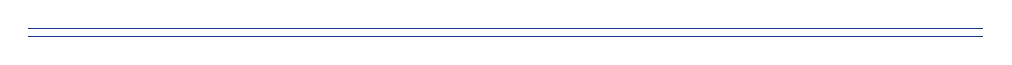
\begin{tikzpicture}
    \draw[thin, navy] (0,0) -- (\linewidth, 0);
    \draw[thin, navy] (0,-0.1) -- (\linewidth,-0.1);
  \end{tikzpicture}

  \vspace{0.4em}
  
  \begin{tabular}{@{} L{0.3\textwidth} c R{0.3\textwidth} @{}}
    \faEnvelope \hspace{0.1em} \color{softblack} \href{mailto:me@leosharif.com}{me@leosharif.com} & \color{softblack} \multirow{2}{*}{\huge\scshape Leo Sharif} & \faGithub \hspace{0.1em} \color{softblack} \href{https://github.com/Realaiz}{Leo Sharif} \\
    \faPhone \hspace{0.1em} \color{softblack} +61 420-677-719 & & \textcolor{LinkedinBlue} \faLinkedinSquare \hspace{0.1em} \color{softblack} \href{https://www.linkedin.com/in/leo-sharif-1a6866193/}{Leo Sharif} \\
    & \color{softblack} \normalsize \color{subtextgray} Mathematics \& Finance & \faHome \hspace{0.1em} \color{softblack} \href{https://leosharif.com}{leosharif.com} \\
  \end{tabular}

  \vspace{0.4em}

  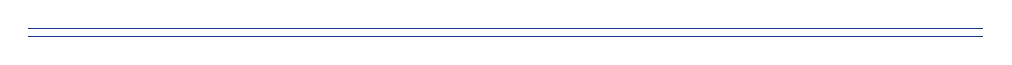
\begin{tikzpicture}
    \draw[thin, navy] (0,0) -- (\linewidth,0);
    \draw[thin, navy] (0,-0.1) -- (\linewidth,-0.1);
  \end{tikzpicture}
\end{center}


% Education Section
\section{education}
\textbf{Bond University} \hfill {Gold Coast, QLD} \\
\indent \textit{\color{subtextgray}B. Actuarial Science, Major in Finance} \hfill \textit{\color{subtextgray} Feb 2022 - Jul 2024}
\begin{itemize}[noitemsep, topsep=0em, left=0.8em]
  \item 75\% Major WAM, Investment Group, Actuarial Society, Actuaries Institute Completion: CS, CM, CB
  \item Coursework: Mathematical Statistics, Stochastic Processes, Econometrics, Finance Mathematics, Portfolio Analysis, Survival Analysis, Risk Management, Financial Models, Game Theory, Survival Analysis
\end{itemize}

\textbf{Academy of Interactive Technology} \\
\indent \textit{\color{subtextgray}Diploma of Full Stack Development} \hfill \textit{\color{subtextgray} Aug 2020 - Jun 2021}
\begin{itemize}[topsep=0em, left=0.8em]	
  \item 78\% WAM, Developed a real estate portfolio management tool, showcasing strong problem-solving skills and industry-standard security practices.
\end{itemize}

\vspace{1em}

\section{work \& experience}

\vspace{0.20em}

\textbf{Nabla} \hfill {Gold Coast, QLD} \\
\indent \textit{\color{subtextgray}President} \hfill \textit{\color{subtextgray}Feb 2023 - May 2024}
\begin{itemize}[noitemsep, topsep=0em, left=0.8em]
  \item Founded the Quantitative Finance Society to meet demand for quantitative investment analysis; onboarded a dedicated team to drive objectives and promote growth.
  \item	Developed a heat map for option strike prices using Python and C++ to create an interactive, engaging dashboard for members.
  \item Explored the usage of ESG factors in quantitative analysis.
\end{itemize}

\textbf{Sitesec} \hfill {Gold Coast, QLD} \\
\indent \textit{\color{subtextgray}Systems Engineer} \hfill \textit{\color{subtextgray}Nov 2022 - Jul 2023}
\begin{itemize}[noitemsep, topsep=0em, left=0.8em]
  \item Managed databases and ensured data integrity, accuracy, and availability for stakeholders.
  \item	Leveraged data analytical techniques to map and plan construction projects, optimising resource allocation and project timelines.
  \item Worked with senior developers on Convolutional Neural Networks to identify security risks at a 20\% higher rate.
\end{itemize}



\textbf{Eante} \hfill {Brisbane, QLD} \\
\indent \textit{\color{subtextgray}Software Development Intern} \hfill \textit{\color{subtextgray}Jan 2021 - May 2021}
\begin{itemize}[noitemsep, topsep=0em, left=0.8em]
  \item Developed a micro interest-earning system with visual representations to encourage saving habits.
  \item	Gained exposure to development of explosion mapping software for an international mining project.
\end{itemize}

\vspace{1em}

\section{Competitions \& Research}

\noindent
\begin{minipage}{0.15\textwidth}
    \includegraphics[width=\linewidth]{icons/SIG-icon}
\end{minipage}%
\begin{minipage}{0.8\textwidth}
    6th @ 2024 Susquehanna Algothon - Designed trading algorithms for a universe of 50 stocks with a sharpe of 2.14. (\$9,000 Prize Pool)
\end{minipage}

\vspace{1em}

\section{skills}

\hspace{-2.5em} \begin{tabular}{>{\raggedright}p{0.1\textwidth} p{0.9\textwidth}}
  \textbf{Languages} & \includegraphics[height=1em]{icons/python-icon} Python, 
\includegraphics[height=1em]{icons/r-icon} R, \includegraphics[height=1em]{icons/cpp-icon}  C++, 
\includegraphics[height=1em]{icons/w3_html5-icon}\includegraphics[height=1em]{icons/w3_css-icon}\includegraphics[height=1em]{icons/js-icon} HTML/CSS/JS, 
\includegraphics[height=1em]{icons/typescriptlang-icon} TypeScript, 
\includegraphics[height=1em]{icons/amazon_aws-icon} AWS, \includegraphics[height=1em]{icons/ruby-lang-icon} Ruby \\
  \textbf{Data} & 
\includegraphics[height=1em]{icons/Pandas} Pandas, \includegraphics[height=1em]{icons/scikit-learn} Scikit, \includegraphics[height=1em]{icons/Ploty} Plotly, \includegraphics[height=1em]{icons/seaborn-icon} seaborn, \includegraphics[height=1em]{icons/pytorch-icon} PyTorch, \includegraphics[height=1em]{icons/node-icon} \includegraphics[height=1em]{icons/react-icon} \includegraphics[height=1em]{icons/Next.js} Node/React/Next
\end{tabular}
\vspace{1em}

\section{additional info}

\hspace{-2.5em} \begin{tabular}{>{\raggedright}p{0.1\textwidth} p{0.9\textwidth}}
  \textbf{Interests} & Acting, Gastronomy, Guitar, Piano, Tennis, NFL, NBA, Music, Fashion, Gaming \\
  \textbf{Volunteering} & Certificate in Active Volunteering (III), Litter Drive, Tennis Coach, Tutoring
\end{tabular}



\end{document}



